% !TEX Root = ../proposal.tex

\section[Prior Research]{Research into spacecraft mission design}
\subsection[Reachability Sets]{Orbital transfers via Reachability Sets}

\begin{frame}{Orbital Transfers} % -----------------------------------%
    \begin{itemize}
        \item \Emph{Reachability set} allows for systematic transfer design
        \begin{itemize}
            \item Transfer design on lower dimensional \Poincare surface
            \item Simple method to incorporate effects of low-thrust 
            \item Avoids the issue of determining initial conditions
        \end{itemize}
    \pause
        \item Alleviates many issues with previous approaches
        \begin{itemize}
            \item Initial states chosen from from the reachable set
            \item Indirect optimal control vs. direct optimal control
            \item Reachability set gives bounds on motion
        \end{itemize}    
    \end{itemize}

  \note[itemize]{
    \item here we introduce some of our previous work that aims to apply geometric mechanics to the design of trajectories around asteroids
    \item Reachability set avoids the need to pick initial conditions
    \item We compute on a lower dimensional surface
  }
\end{frame} %--------------------------------------%

\subsubsection[Dynamic Systems Theory Review]{Dynamic Systems}

\begin{frame}{\Poincare map}
\begin{itemize}
    \item Intersection of a periodic orbit with a lower dimensional subspace
    \pause
        \begin{itemize}
            \item  \Emph{\Poincare section} - discrete map between intersections
        \end{itemize}
        \pause
    \item Useful for investigating the stability and structure 
    \pause
    \item Define a \Poincare section \( \Sigma \) 
        \begin{itemize}
            \item Used for initial and target periodic orbits
            \item Subspace for the \Emph{reachability set}
        \end{itemize}
\end{itemize}

\begin{center}
    \begin{scaletikzpicturetowidth}{0.3\textwidth}
    \begin{tikzpicture}[tdplot_main_coords,
          poincare/.style={opacity=.2,very thick,fill=blue},
          orbit/.style={very thick,black},
          orbit hidden/.style={very thick,dashed},
          grid/.style={very thin,gray!50},
          axis/.style={->,blue,thick},scale=0.6]

        % draw periodic orbit
        \onslide<4->{
            % draw a periodic orbit
            \coordinate (center) at (0,0,2);
            \node[above left] (x0) at (0,2,2) {\(\vecbf{x}_0\)};
            \filldraw (0,2,2) circle (3pt);
        }

        \onslide<5->{
            \tdplotdrawarc[orbit hidden]{(center)}{2}{90}{190}{}{};
            \tdplotdrawarc[orbit,<-]{(center)}{2}{-170}{90}{}{};
        }

        \onslide<6->{
            % nodes for the poincare section
            \node[label=above:\(\Sigma\)] (upper_right) at (0,5,5) {};
            \node[] (upper_left) at (0,1,5) {};
            \node[] (lower_left) at (0,1,0) {};
            \node[] (lower_right) at (0,5,0) {};

            % draw poincare section
            \draw[poincare] (upper_right.center) -- (upper_left.center) -- (lower_left.center) -- (lower_right.center) -- (upper_right.center);
        }
        
        \onslide<7->{
            \node[below right] (x1) at (0,3,2) {\(\vecbf{x}_1\)};
            \filldraw (0,3,2) circle (3pt);
        }

        \onslide<8->{
            \tdplotdrawarc[orbit hidden]{(center)}{3}{90}{199}{}{};
            \tdplotdrawarc[orbit,<-]{(center)}{3}{-161}{90}{}{};
        }
    \end{tikzpicture}
    \end{scaletikzpicturetowidth}
\end{center}

\note[itemize]{
    \item Here we present a review of the key components of dynamical systems theory
    \item we start with some initial condition \( \vecbf{x}_0\) on a periodic orbit
    \item we then define a section \( \Sigma \) transverse to this flow
    \item we can use the successive iterations of these periodic orbits to study the dynamics of the system on a lower dimensional surface.
    \item Periodic orbits show up as fixed points while sinks/sources will have a distinctly different behavior
}
\end{frame}

\begin{frame}{Reachability Set}

\begin{itemize}
    \item Set of states achievable from a given initial condition over fixed \( t_f \) s.t. maximum control constraint
    \[
        R( \vecbf{x}_0, \mathcal{U} , t_f) = \braces{ \vecbf{x}_f \subseteq \mathcal{X} | \exists \vecbf{u} \in \mathcal{U}, \vecbf{x}(t_f) = \vecbf{x}_f }
    \]
    \pause
    \item Directly derivable from optimal control
    \item Frequently used for safety planning, e.g. air traffic avoidance
    \pause
    \item Extend to the design of orbital transfers
\end{itemize}

\note[itemize]{
    \item Given the state of an aircraft, we can predict where it can end up over a fixed amount of time.
    \item To avoid any possibility of collision, we want to make sure these sets do not intersect
}
\end{frame}

\begin{frame}{Reachability Set on \Poincare section} % -----------------------------------%

\begin{itemize}
    \item Generate the reachability set on a \Poincare section, \( \Sigma \)
    \item Control input is chosen to enlarge the reachable set
\end{itemize}

\begin{center}
    \begin{tikzpicture}[tdplot_main_coords,
      poincare/.style={opacity=.2,very thick,fill=blue},
      orbit/.style={very thick,black},
      orbit hidden/.style={very thick,dashed},
      grid/.style={very thin,black},
      axis/.style={->,blue,thick},
      reachability/.style={thick,blue}]

    % draw axes
    % \draw[axis] (0,0,0) -- (5,0,0) node[anchor=west]{$x$};
 %    \draw[axis] (0,0,0) -- (0,5,0) node[anchor=west]{$y$};
 %    \draw[axis] (0,0,0) -- (0,0,5) node[anchor=west]{$z$};

    % nodes for the poincare section
    \node[] (upper_right) at (0,5,5) {};
    \node[] (upper_left) at (0,1,5) {};
    \node[] (lower_left) at (0,1,0) {};
    \node[] (lower_right) at (0,5,0) {};

    \onslide<2->{
        % draw poincare section
        \draw[poincare] (upper_right.center) -- (upper_left.center) -- (lower_left.center) -- (lower_right.center) -- (upper_right.center);
        \node[label=above:\(\Sigma\)] at (upper_right) {};
        }

    % draw a periodic orbit
    \coordinate (center) at (0,0,2);
    \node[] (x0) at (0,3,2) {};
    \onslide<3>{
        \node[label=left:\(\vecbf{x}_0\)] at (x0) {};
        
    }
    \onslide<4->{
        \filldraw (x0) circle (3pt);
        \node[label=below:\(\vecbf{x}_n\)] at (x0) {};
    }

    \onslide<4-5>{
        \tdplotdrawarc[orbit hidden]{(center)}{3}{90}{200}{}{};
        \tdplotdrawarc[orbit,<-]{(center)}{3}{-160}{90}{}{};
        }

    \coordinate (reach) at (0,4.5,2);
    \tdplotsetthetaplanecoords{90}

    % draw poincare angles
    \onslide<5->{
        \draw[tdplot_rotated_coords,grid] (x0) -- (reach);
        \draw[tdplot_rotated_coords,grid] (x0) -- ++(-45:1.5);
        \tdplotdrawarc[tdplot_rotated_coords,grid]{(x0)}{0.5}{-45}{90}{above}{\(\phi\)};
        }


   % draw terminal state on reachability set
    \onslide<6->{
        \node[tdplot_rotated_coords,label=above:\(\vecbf{x}_f\)] (xf) at ($ (x0)+(-45:1.5) $) {};
        \filldraw (xf) circle (3pt);
        }

    \onslide<7->{
        \node[tdplot_rotated_coords,label=below:\(J\)] at (xf) {};
        }

    \onslide<8->{
        \tdplotdrawarc[tdplot_rotated_coords,reachability]{(x0)}{1.5}{0}{360}{}{};
    }
    
\end{tikzpicture}
\end{center}

\note[itemize]{
    \item We combine both reachability and the \Poincare section to design transfers
    \item again we define our section \( \Sigma\)
    \item choose an initial state that is on \( \Sigma \)
    \item propogate without any control input from \( \vecbf{x}_0 \) to \( \vecbf{x}_n\)
    \item by adding the control input the terminal state will be something different at \( \vecbf{x}_f\)
    \item we define the distance between \( \vecbf{x}_n\) and \(\vecbf{x}_f\) with \( J \) - want to maximize this
    \item Repeat this computation many times for a variety of angles \( \phi\)
}
\end{frame} %--------------------------------------%

\subsection[Formulating the optimal control problem]{Optimal Control Problem}

\begin{frame}{Optimal Control Problem}
\begin{itemize}
    \item Reachability defined as distance between controlled and uncontrolled states
        \[
            J = -\frac{1}{2} \left( \vecbf{x}(t_f) - \vecbf{x}_{n}(t_f)\right)^T 
            Q
            \left( \vecbf{x}(t_f) - \vecbf{x}_{n}(t_f)\right) 
        \]
    
    \pause
    \item Terminal constraints - \( \vecbf{m}_i(\vecbf{x}_f) = 0\) ensures \( \Sigma \) intersection
    \pause
    \item Control constraint used to emulate realistic system
        \[
            c(\vecbf{u}) = \vecbf{u}^T \vecbf{u} - u_m^2 \leq 0 
        \]
\end{itemize}

\note[itemize]{
    \item Formulate the reachability in terms of an optimal control problem
}
\end{frame}

\begin{frame}{Shooting Method}
\begin{itemize}
    \item Shooting method used to solve boundary value problem
    \item Convergence is difficult with with single shooting
    \item<6-> Multiple shooting sub-divides the total interval
\end{itemize}

\only<2-5>{
\begin{scaletikzpicturetowidth}{\textwidth}
    \begin{tikzpicture}[scale=\tikzscale]
        \onslide<2->{
            \node[label=west:\(\vecbf{x}\)] (x0m) at (0,5) {};
            \node[] (xnm) at (20,5) {};
    
            \node[label=below:\(t_0\)] (t0) at (0,0) {};
            \node[label=below:\(t_f\)] (tf) at (20,0) {};

            \draw [<->,thick] (tf.center) -- (t0.center) -- (x0m.center);

            % nodes for each subsegment
            \node[label=left:\(\vecbf{x}_0\)] (x0) at (0,1) {\pgfuseplotmark{*}};
            \node[label=below left:\(\vecbf{\lambda}_0\)] at (x0) {};
            \node[label=right:\(\vecbf{x}_f\)] (xnminus) at (20,3) {\pgfuseplotmark{*}};
            \node[label=below right:\(\vecbf{\lambda}_f\)] at (xnminus) {};
        }


        % shooting attempts
        \onslide<3->{
            \draw [->,dashed] (x0.center) to [bend left=20] ($ (xnminus.center)+(0,1) $);
        }
        \onslide<4->{
            \draw [->,dashed] (x0.center) to [bend right=10] ($ (xnminus.center)+(0,-1) $);
        }
        % final correct shooting path
        \onslide<5->{
            \draw [->] (x0.center) to [bend left=10] (xnminus.center);
        }
    \end{tikzpicture}
\end{scaletikzpicturetowidth}
}

\only<6->{
\begin{scaletikzpicturetowidth}{\textwidth}
        \begin{tikzpicture}[scale=\tikzscale]
    % \draw[help lines] (0,0) grid (20,5) ; %grid
    \node[label=west:\(\vecbf{x}\)] (x0m) at (0,5) {};
    \node[] (x1m) at (5,5) {};
    \node[] (x2m) at (10,5) {};
    \node[] (x3m) at (15,5) {};
    \node[] (xnm) at (20,5) {};

    \node[label=below:\(t_0\)] (t0) at (0,0) {};
    \node[label=below:\(t_n\)] (tn) at (20,0) {};

    % nodes for each subsegment
    \node[label=left:\(\vecbf{x}_0\)] (x0) at (0,1) {\pgfuseplotmark{*}};
    \node[label=below left:\(\vecbf{\lambda}_0\)] at (x0) {};

    \node[label=right:\(\vecbf{x}_n\)] (xnminus) at (20,3) {\pgfuseplotmark{*}};
    \node[label=below right:\(\vecbf{\lambda}_n\)] at (xnminus) {};

    % draw axes
    \draw [<->,thick] (tn.center) -- (t0.center) -- (x0m.center);


    \onslide<7->{
        
        \node[label=below:\(t_1\)] (t1) at (5,0) {};
        \node[label=below:\(t_2\)] (t2) at (10,0) {};
        \node[label=below:\(t_{n-1}\)] (t3) at (15,0) {};
        
                \node[label=right:\(\vecbf{x}_1^{-}\)] (x1minus) at (5,2) {\pgfuseplotmark{*}};
        \node[label={135:\(\vecbf{x}_1^{+}\)}] (x1plus) at (5,3) {\pgfuseplotmark{o}};

                \node[label=right:\(\vecbf{x}_2^{-}\)] (x2minus) at (10,2) {\pgfuseplotmark{*}};
        \node[label={135:\(\vecbf{x}_2^{+}\)}] (x2plus) at (10,3) {\pgfuseplotmark{o}};

                \node[label=right:\(\vecbf{x}_{n-1}^{-}\)] (x3minus) at (15,2) {\pgfuseplotmark{*}};
        \node[label={135:\(\vecbf{x}_{n-1}^{+}\)}] (x3plus) at (15,3) {\pgfuseplotmark{o}};
        % draw segement dividers
        \draw [dashed,thick] (t1.center) -- (x1m.center);
        \draw [dashed,thick] (t2.center) -- (x2m.center);
        \draw [dashed,thick] (t3.center) -- (x3m.center);
        \draw [dashed,thick] (tn.center) -- (xnm.center);
    }

    \onslide<8->{

        \draw [->] (x0.center) to [bend left=30] (x1minus.center);
    }

    \onslide<9->{

        \draw [->] (x1plus.center) to [bend left=30] (x2minus.center);
    }

    \onslide<10->{
        % dotted lines here

        \draw[decorate sep={2mm}{10mm},fill] (x2plus.east) to [bend left=30] (x3minus.west);
    }

    \onslide<11->{

        \draw [->] (x3plus.center) to [bend left=30] (xnminus.center);
    }


\end{tikzpicture}
\end{scaletikzpicturetowidth}
}
\note[itemize]{
    \item The euler lagrange equations transforms from an optimal control problem to a two point boundary value problem
    \item in the shooting method we try to choose initial conditions \( \vecbf{\lambda}_0\) to satisfy some set of terminal conditions
    \item Again it's prone to sensitivty so we instead use a multiple shooting method 
    \item We divide the time interval into smaller sub segments and add additional interior constraints to ensure a continuous trajectory
    \item Each sub stage is then a smaller single shooting approach
    \item this ends up reducing the sensitivity of the terminal states to variations of the intial conditions
}
\end{frame}

\begin{frame}{Solving the Optimal Control Problem}

\begin{itemize}
    \item Shooting method to solve the necessary conditions
    \pause
    \item Approximate the reachable set via \( \phi_i \) 
    \begin{itemize}
        \item Parameterize a direction on \( \Sigma \)
    \end{itemize}
    \pause
    \item From the reachable set we chose the state which minimizes \( d \) 
    \item Compute another reachable set if target is not feasible
\end{itemize}
\[
    d = \norm{\vecbf{x}_f - \vecbf{x}_t} 
\]

\end{frame}

% results from 2015 AAS
\subsection[Transfer examples using Reachability Sets]{Transfer Examples}

\begin{frame}[t]{Orbital Transfers via Reachability Sets}
    \begin{itemize}
        \item Numerical simulations in two different environments
        \begin{itemize}
            \item Planar Circular Restricted Three Body Problem
            \item Restricted Two Body Problem 
        \end{itemize}
        \pause
        \item Dynamics are related but vary in complexity
        \begin{itemize}
            \item Planar vs. Three Dimensional
            \item Gravitational Potential
            \item Both defined in a rotating reference frame
        \end{itemize}
    \end{itemize}

\note[itemize]{
    \item here we show some examples of using this approach to design transfers in two different dynamic enviornments
}
\end{frame}

\subsubsection[Circular Restricted Three Body Problem]{Three Body Problem}

\begin{frame}%--------------------------------------------%
\frametitle{Three Body Problem}
    \begin{itemize}
        \item Transfer from \( L_1 \) orbit to periodic orbit near the Moon
        \item Bounded control input and fixed time horizon
    \end{itemize}
    \visible<2>{
        \begin{center}
            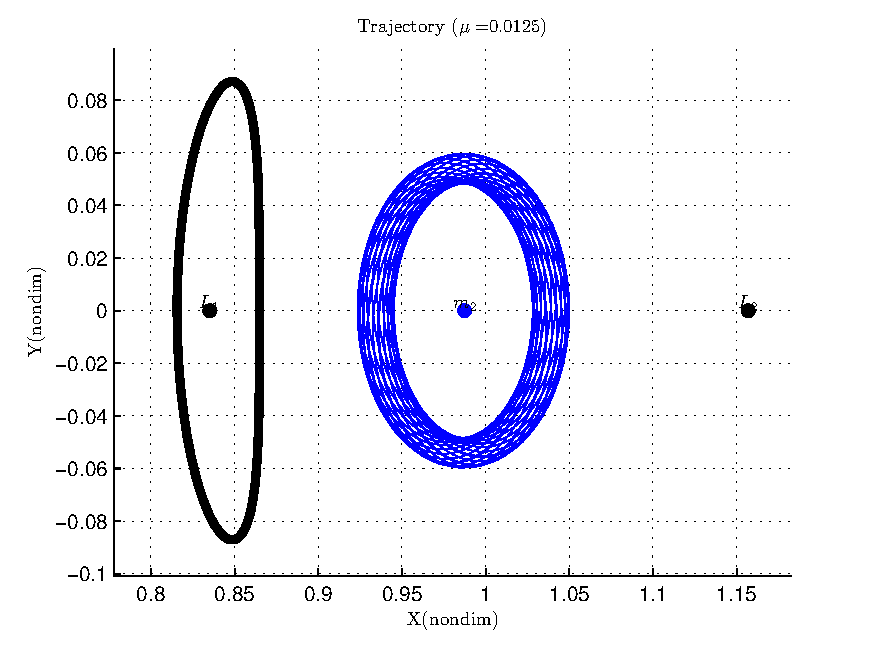
\includegraphics[width=0.7\textwidth,height=0.7\textheight,keepaspectratio]{2015AAS/moon_orbit.pdf}
        \end{center}
        }
    
    \note[itemize]{
        \item Introduce problem and initial and terminal orbits. 
        \item Earth is way off to the left with the Moon at the center
        \item Possible use as a communication array
        \item Might actually be a distant retrograde orbit
        }
\end{frame} %--------------------------------------------%

\begin{frame}%------------------------------------------------%
    \frametitle{Reachable Set Transfer}
    \begin{itemize}
        \item Approximate the reachable set on the \Poincare section
        \begin{itemize}
            \item Generate many optimal solutions
        \end{itemize}
        \item<3-> Intersection point used to generate a transfer
        \begin{itemize}
            \item Shorter time of flight than uncontrolled dynamics
        \end{itemize}
    \end{itemize}
    \begin{center}
        \only<1-2>{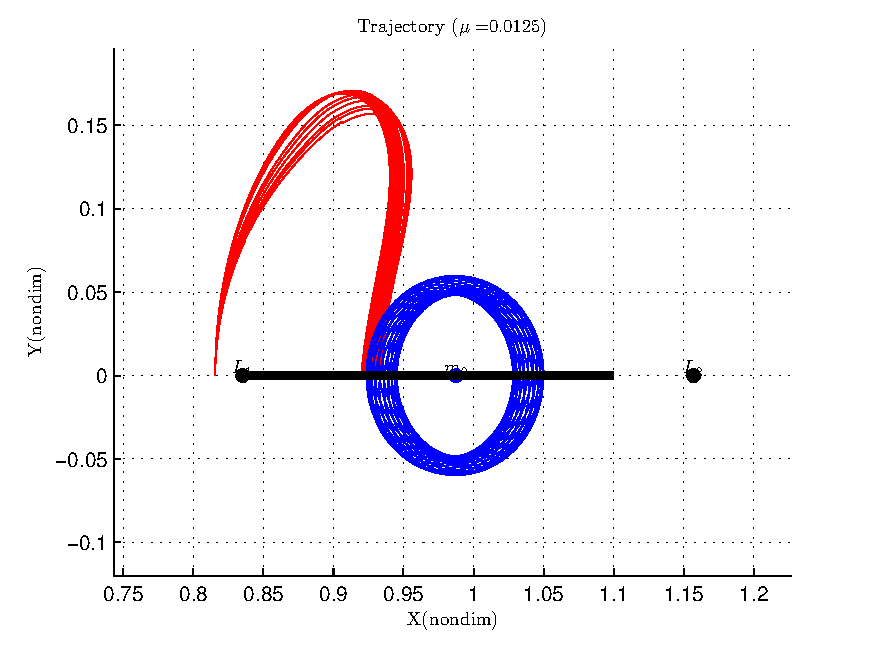
\includegraphics[width=0.5\textwidth,height=0.7\textheight,keepaspectratio]{2015AAS/reach_trajectory}~}
        \only<3->{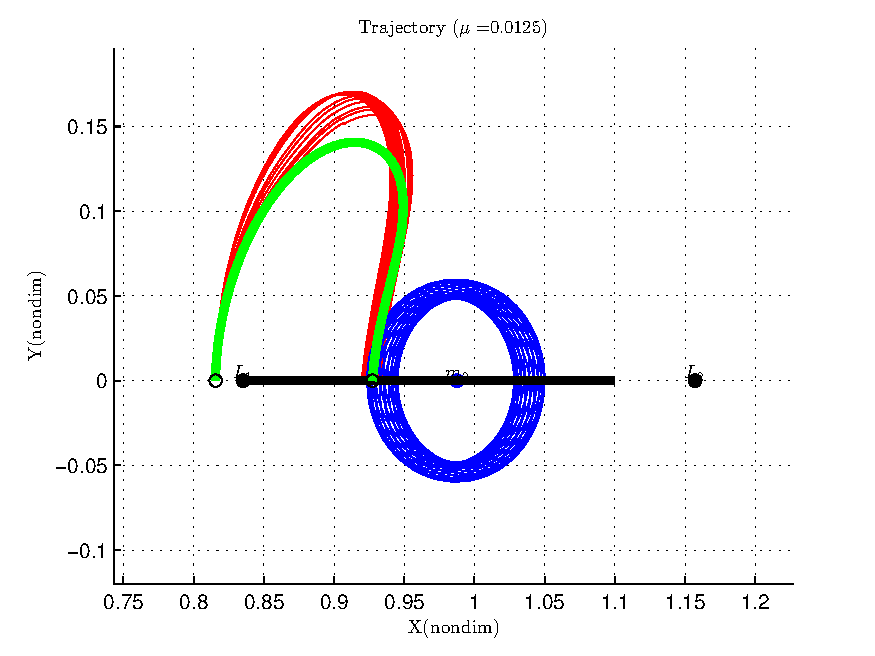
\includegraphics[width=0.5\textwidth,height=0.7\textheight,keepaspectratio]{2015AAS/reach_transfer}~}
        \only<2-3>{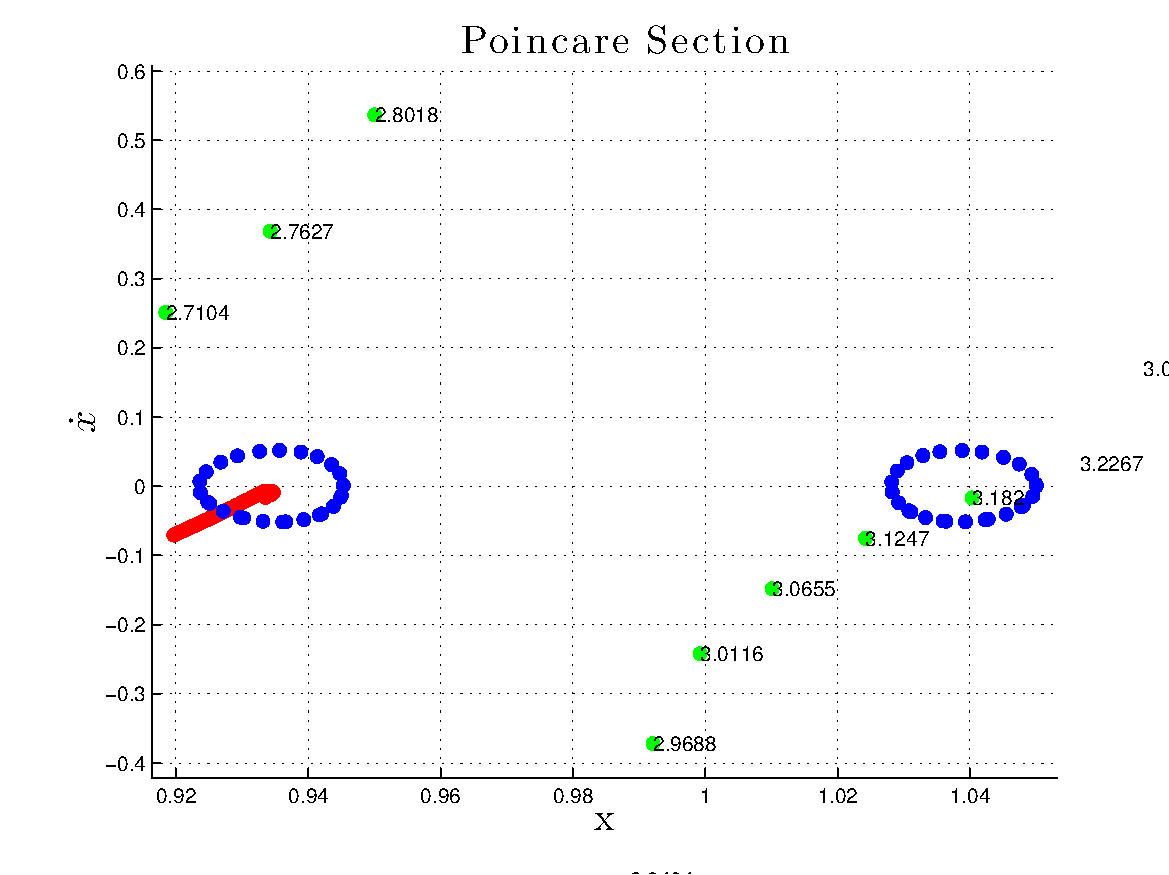
\includegraphics[width=0.5\textwidth,height=0.7\textheight,keepaspectratio]{2015AAS/poincare_compare}} 
    \end{center}
    
    \note[itemize]{
        \item Compare to reachable set approach
        \item Shorter time of flight
        \item Multiple shooting to solve TPBVP
        Vary \( \theta\) to change direction on section
        Linear interpolation to determine intersection on Poincar\'e section
        \item Only one reachabile set computation is required
        }
\end{frame} %--------------------------------------------------%

\begin{frame}{Geostationary  transfer} %----------------------------------------------------%
    \begin{itemize}
           \item Transfer from geostationary orbit to a \( L_1\) periodic orbit 
           \item Multiple iterations of reachable set required for transfer
    \end{itemize}

    \begin{center}
       \only<1>{
       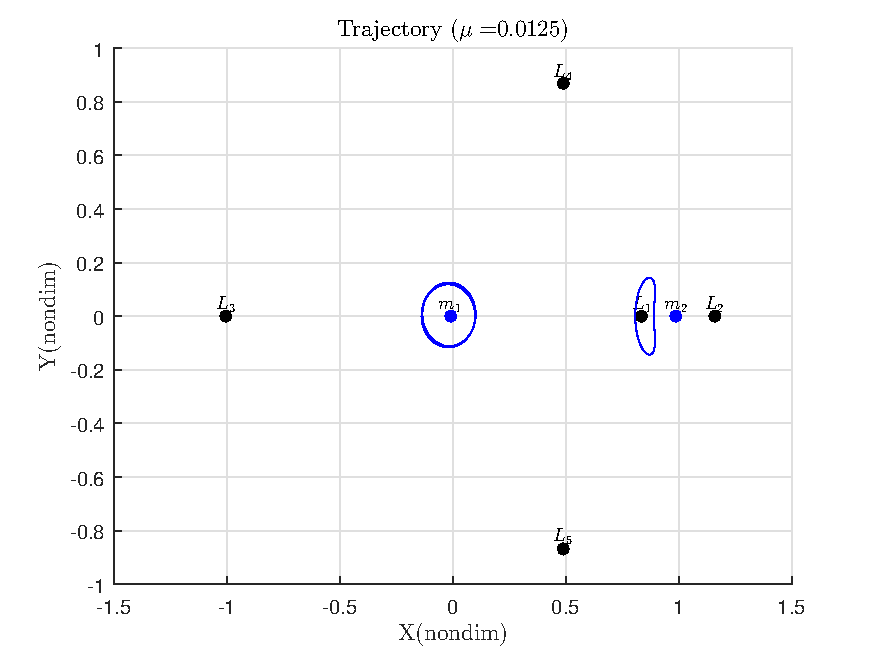
\includegraphics[width=0.5\textwidth,height=0.7\textheight,keepaspectratio]{figures/2015ACTA/initial_final.pdf}~
       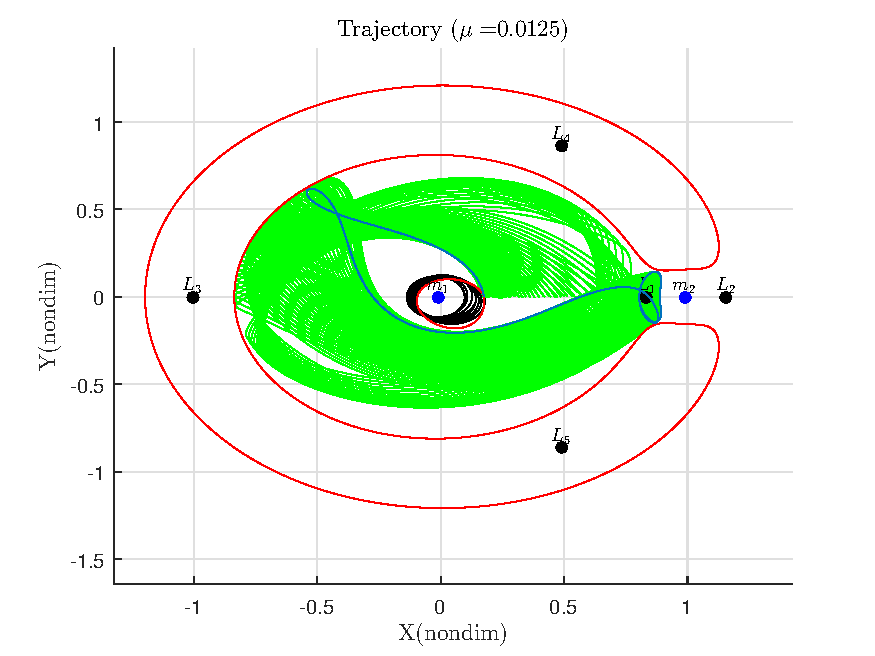
\includegraphics[width=0.5\textwidth,height=0.7\textheight,keepaspectratio]{figures/2015ACTA/geo_transfer_full.pdf} 
       }

       \only<2>{
       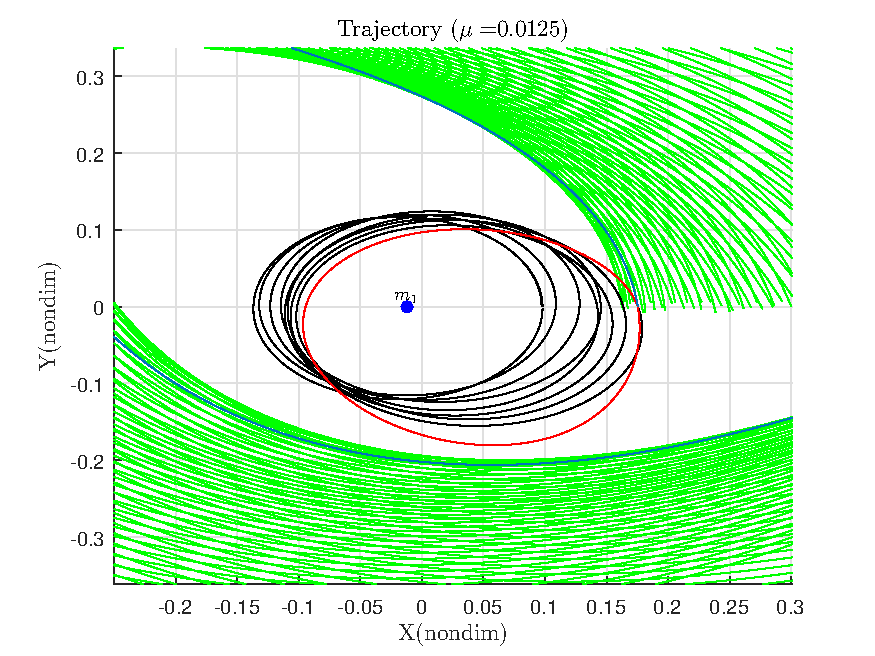
\includegraphics[width=0.5\textwidth,height=0.7\textheight,keepaspectratio]{figures/2015ACTA/geo_transfer_zoom.pdf}~
       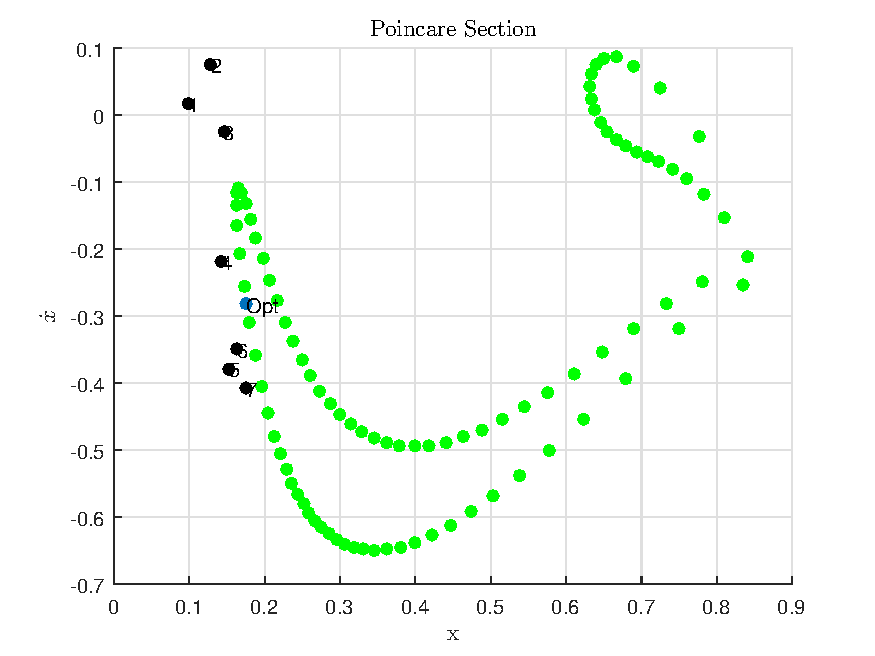
\includegraphics[width=0.5\textwidth,height=0.7\textheight,keepaspectratio]{figures/2015ACTA/poincare.pdf}
       }
    \end{center}

\note[itemize]{
    \item The green trajectories are the invariant manifolds and require no control input to traverse large regions of the phase space
}
\end{frame} %--------------------------------------------%

\subsubsection[Transfers about 4769 Castalia]{Asteroid transfers}

% Results from 2016 AAS
\begin{frame}{Transfer Objective} %-----------------------------%

\begin{itemize}
    \item Goal is to transfer between two equatorial periodic orbits
    \item Typical scenario during study of an asteroid
\end{itemize}

\begin{center}
    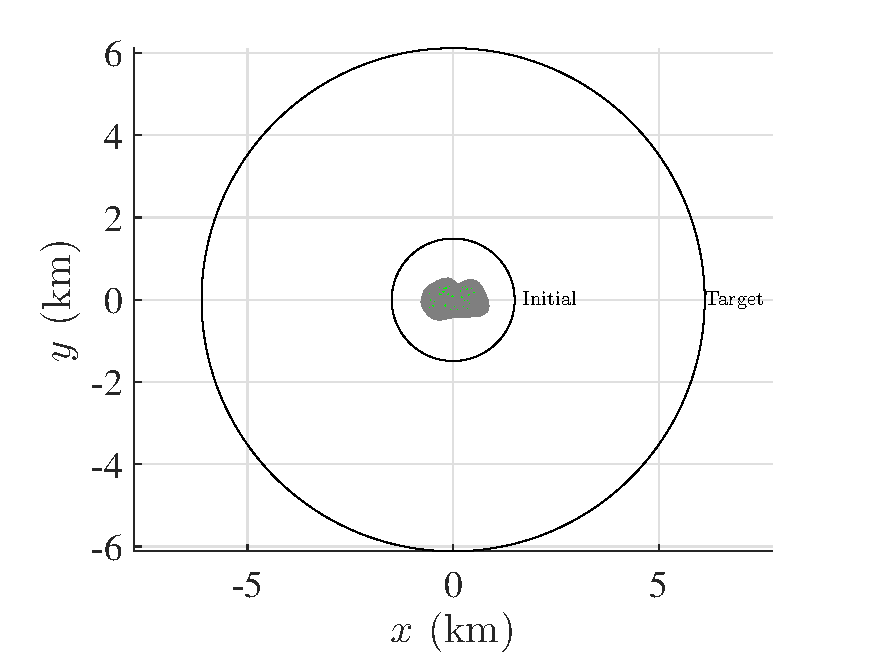
\includegraphics[width=0.5\textwidth,height=0.7\textheight,keepaspectratio]{figures/2016AAS/initial_transfer.pdf}~
    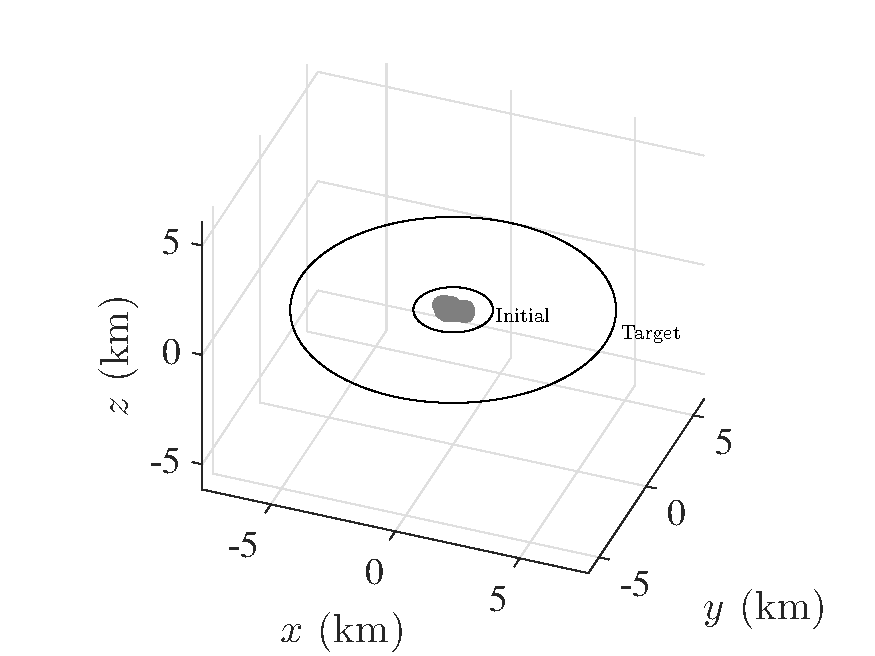
\includegraphics[width=0.5\textwidth,height=0.7\textheight,keepaspectratio]{figures/2016AAS/initial_transfer_3d.pdf}
\end{center}

\note[itemize]{
    \item Now we apply the same methodology to transfers about asteroids
}
\end{frame}%-----------------------------%

\begin{frame}{Simulation}

\begin{itemize}
    \item Generate the reachability set through discretization of \( \phi_i \)
    \item Visualize \( \Sigma \in \R^4 \) through the use of two 2-D sections
    \pause
    \item Control input allows for depature from natural dynamics
\end{itemize}

\begin{center}
    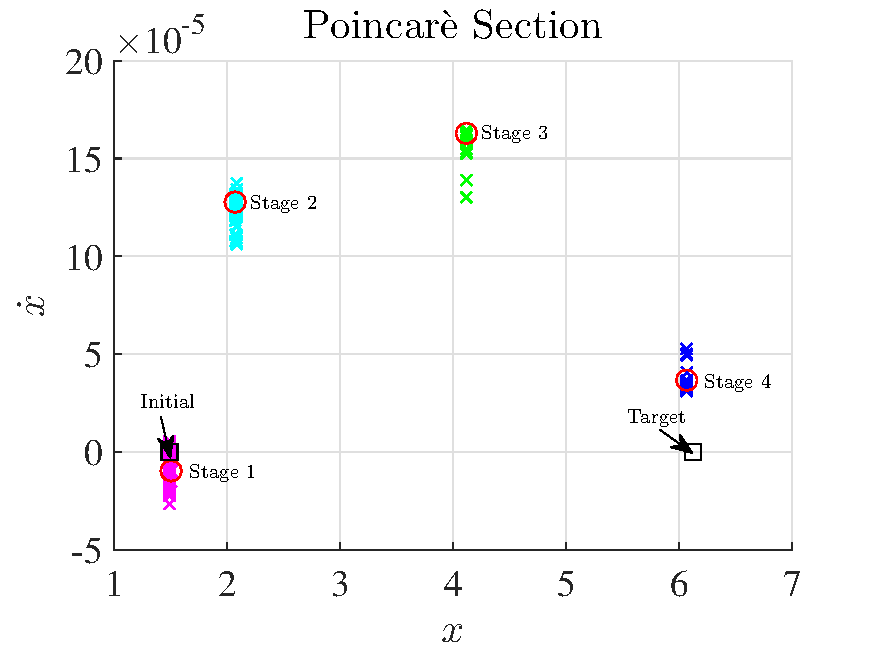
\includegraphics[width=0.5\textwidth,height=0.7\textheight,keepaspectratio]{figures/2016AAS/poincare_xvsxdot.pdf}~
    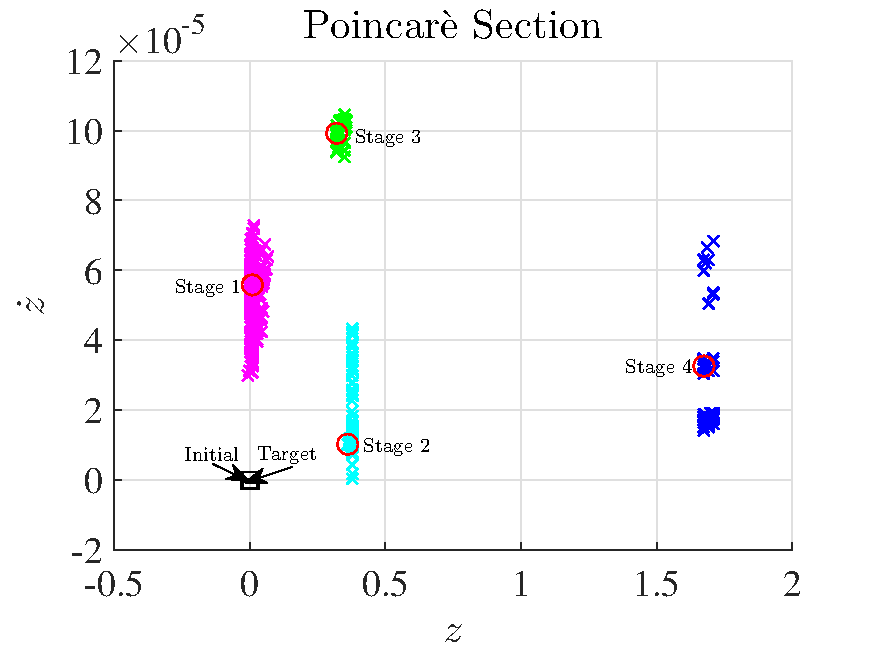
\includegraphics[width=0.5\textwidth,height=0.7\textheight,keepaspectratio]{figures/2016AAS/poincare_zvszdot.pdf}
\end{center}

\note[itemize]{
    \item This \( \Sigma \) is different than before because we're no longer dealing with a planar orbit
    \item We visualize \( \R^4\) using two two-dimensional plots
}
\end{frame}

\begin{frame}{Transfer Simulation}
    \begin{itemize}
        \item Four iterations of the reachable state to meet the target set
        \item Final transfer is computed with a fixed terminal state constraint
    \end{itemize}

    \begin{center}
        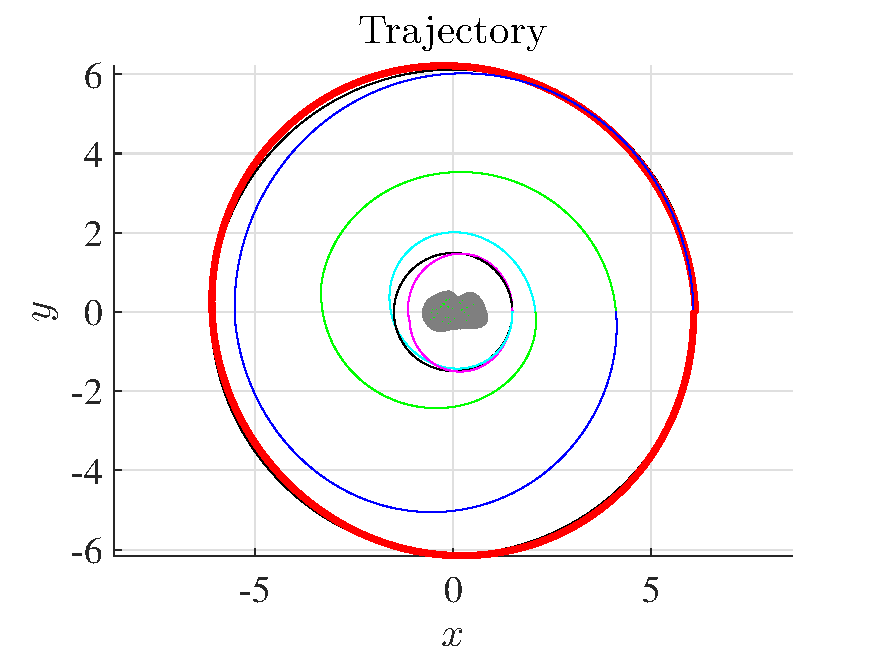
\includegraphics[width=0.5\textwidth,height=0.7\textheight,keepaspectratio]{figures/2016AAS/trajectory.pdf}~
        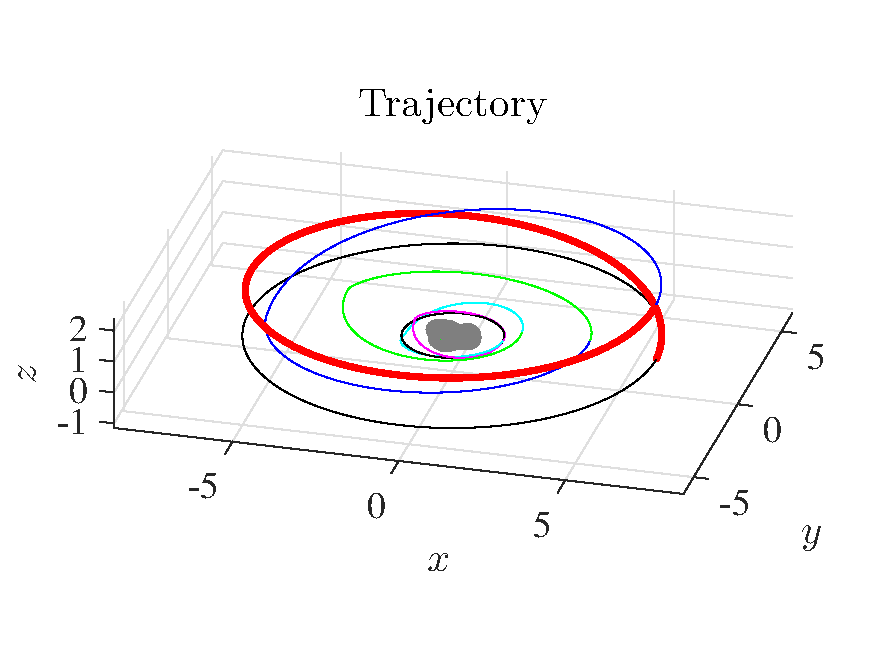
\includegraphics[width=0.5\textwidth,height=0.7\textheight,keepaspectratio]{figures/2016AAS/trajectory_3d.pdf}
    \end{center}

\end{frame}

\begin{frame}{Complete transfer}
\begin{itemize}
    \item We visualize the trajectory in body and inertial frames
\end{itemize}

\begin{center}
  \animategraphics[controls,autoplay,loop,width=0.5\textwidth,height=0.7\textheight,keepaspectratio]{60}{animation/2016AAS/body/IMG}{00500}{01499}~\hfill
  \animategraphics[controls,autoplay,loop,width=0.5\textwidth,height=0.7\textheight,keepaspectratio]{60}{animation/2016AAS/inertial/IMG}{00500}{01499}
\end{center}

\note[itemize]{
    \item we have the body frame on the left and the inertial frame on the right
}
\end{frame}

\subsection[Autonomous Spacecraft attitude control with obstacles]{Constrained Attitude Control}


% Results from 2016 ACC

\begin{frame}{Spacecraft Orientation}\label{slide:attitude_control} %-----------------------------%

\begin{itemize}

    \item \Emph{Attitude Representation}: rotation matrix from body to inertial frame \hyperlink{slide:attitude_kinematics}{\beamergotobutton{Attitude Kinematics}}
     \[\SO =  \{R\in\R^{3\times 3}\,|\, R^TR=I,\;\mathrm{det}[R]=1\} . \]
    \item Rigid body attitude dynamics:
    \begin{gather*}
        J\dot\Omega + \Omega\times J\Omega = u+W(R,\Omega)\Delta , \quad \dot R = R\hat\Omega .
    \end{gather*}

    \item Sensor and obstacles defined by unit vectors in \( \R^3 \) 
        \begin{itemize}
            \item Body fixed sensor: \( r \in \S^2\)
            \item Inertially fixed hazard: \( v \in \S^2 \)
        \end{itemize} 
    \vs
    \item Hard cone constraint: \( r^T R^T v \leq \cos \theta \)
    
\end{itemize}

\note[itemize]{
    \item Obstacle described as a cone around the direction of avoidance
}
\end{frame}   %-----------------------------%

\begin{frame}{Control Objective} %---------------------------------------%

    \begin{block}{Nonlinear Control Design}
        Design control input \( u \) that stabilizes system from initial attitude \( R_0 \) to desired attitude \( R_d \) while avoiding obstacles
    \end{block}
    \pause
    \vs
    \begin{itemize}
        \item Avoid drawbacks of other approaches 
        \begin{itemize}
            \item \Emph{Geometric control} - analysis is conducted directly on \( \SO \) 
            \item \Emph{Barrier function} - allows for arbitrary amount of constraints
            \item \Emph{Efficient } - real time feedback control
            \item \Emph{Stability} - Lyapunov analysis gives rigourous stability proof
            \item \Emph{Adaptive} - handles system uncertainties
        \end{itemize}
    \end{itemize}
\end{frame}

\begin{frame}{Configuration Error Function} %-----------------------------%
\only<1>{
\begin{itemize}
    \item Error function quantifies ``distance'' to desired attitude
    \begin{align*}
            \Psi(R, R_d) = A(R, R_d) B(R) .
    \end{align*}
    \vs
    \item Combination of attractive and repulsive terms   
\end{itemize}
\begin{gather*}
    A(R, R_d) = \frac{1}{2} \tr{G \left( I - R_d^T R\right)} . \\ \\
    B_i(R) = 1 - \frac{1}{\alpha_i} \ln \left( - \frac{ r^T R^T v_i - \cos \theta_i}{1 + \cos \theta_i}\right) .
\end{gather*}     
}

\only<2>{
    \begin{itemize}
        \item Attractive well at the desired attitude
    \end{itemize}
    \begin{align*}
        A(R,R_d) = \frac{1}{2} \tr{G \left( I - R_d^T R\right)} .
    \end{align*}
    \begin{center} 
        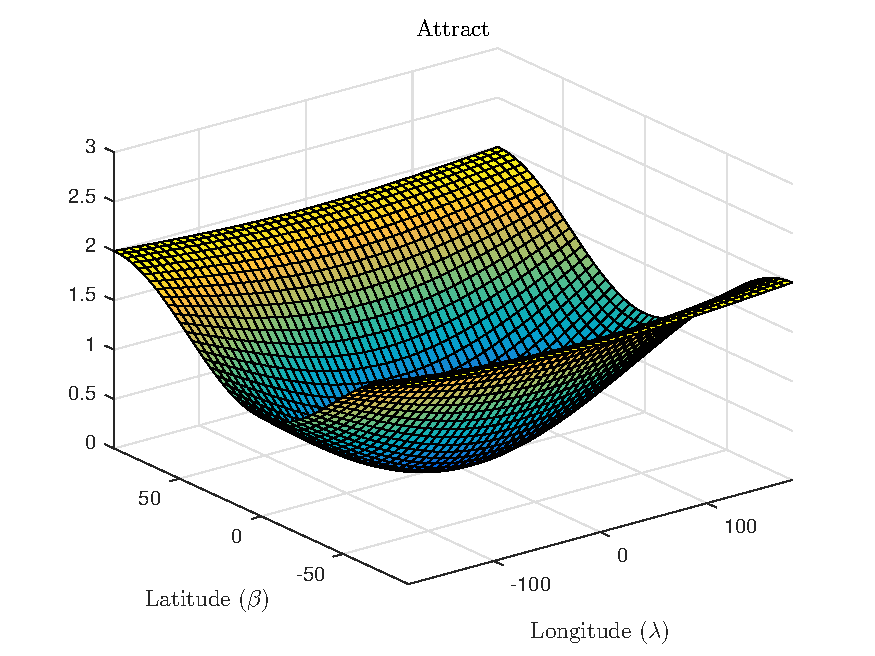
\includegraphics[height=0.6\textheight]{figures/2016ACC/attract_error.pdf}
    \end{center}
}

\only<3>{
    \begin{itemize}
        \item Define a barrier around obstacles
    \end{itemize}
    \begin{align*}
        B_i(R) = 1 - \frac{1}{\alpha_i} \ln \left( - \frac{ r^T R^T v_i - \cos \theta_i}{1 + \cos \theta_i}\right).
    \end{align*}
    \begin{center}
        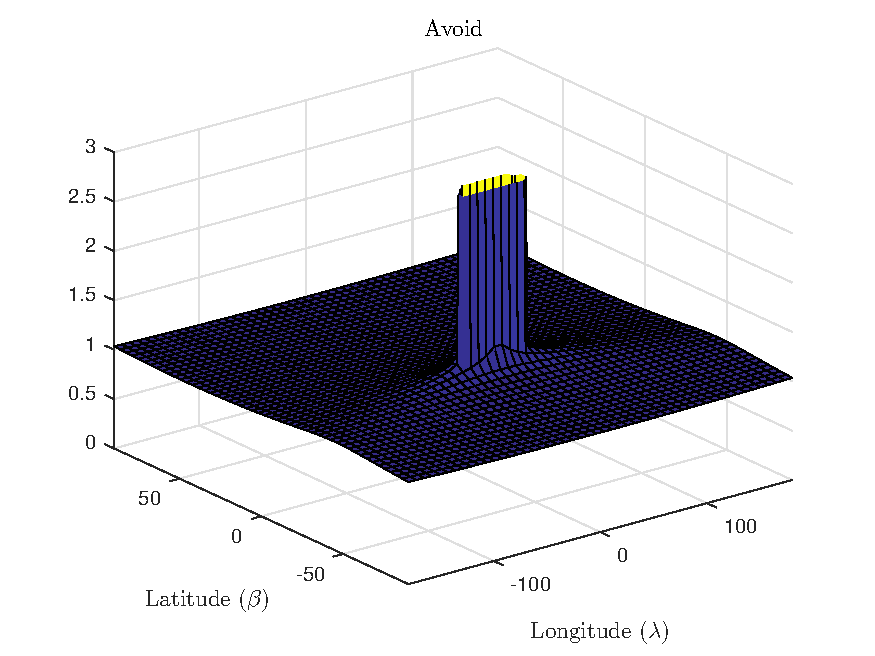
\includegraphics[height=0.6\textheight]{figures/2016ACC/avoid_error.pdf}
    \end{center}

}

\only<4>{
    \begin{itemize}
        \item Configuration error: \( \Psi : \Q \times \Q \to \R \) with control chosen to follow slope of \( \Psi \) to minimum at \( R_d\)
    \end{itemize}
    \begin{align*}
        \Psi(R, R_d) = A(R,R_d) B(R) .
    \end{align*}
    \begin{center}
        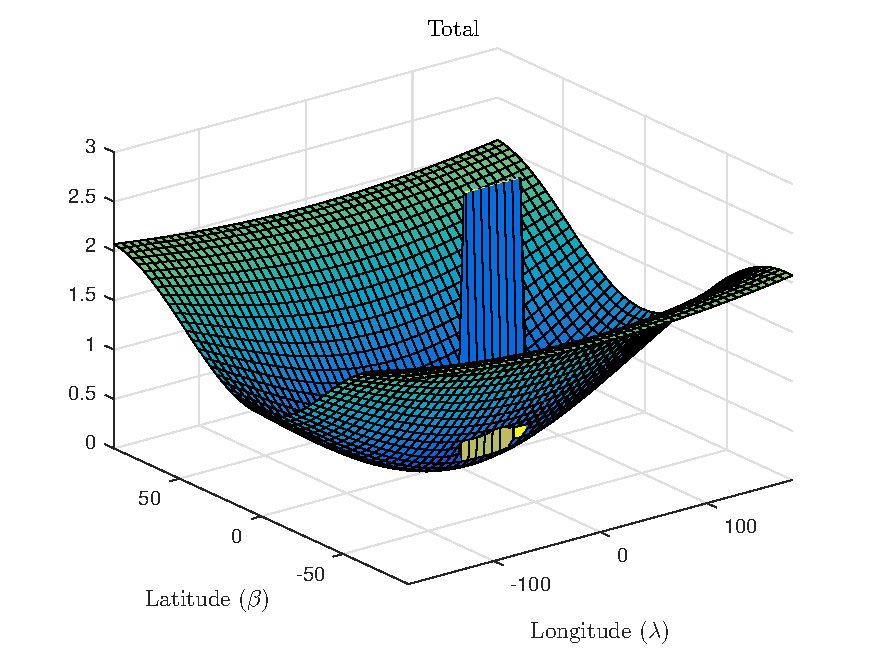
\includegraphics[height=0.6\textheight]{figures/2016ACC/combined_error.pdf}
    \end{center}
}

\note[itemize]{
    \item First step in control design is the selection of an error function
}
\end{frame}   %-----------------------------%

\begin{frame}{Numerical Simulation} %-----------------------------%

\begin{itemize}
    \item Simulate a S/C completing a yaw rotation
    \item Single obstacle in the path of sensor
\end{itemize}

\begin{center}
    \animategraphics[controls,autoplay,loop,width=0.5\textwidth]{8}{animation/2016ACC/single_noavoid/single_noavoid-}{0}{99}~
    \animategraphics[controls,autoplay,loop,width=0.5\textwidth]{8}{animation/2016ACC/single_avoid/single_avoid-}{0}{99}
\end{center}

\end{frame}%-----------------------------%

\begin{frame}{Multiple obstacles}%-------------------------------------%

\begin{itemize}
    \item Easily handle multiple arbitrary constraints 
    \begin{align*}
        \Psi = A(R) \bracket{1 + \sum_i C_i(R)} \quad C_i = B(R) - 1
    \end{align*}
\end{itemize}

\begin{center}
    \animategraphics[controls,autoplay,loop,width=0.5\textwidth,height=0.5\textheight,keepaspectratio]{8}{animation/2016ACC/multiple_avoid/multiple_avoid-}{0}{99}
\end{center}

\end{frame}%---------------------------------------%

\subsubsection[Quadrotor attitude control]{Hardware Implementation}

\begin{frame}{Hexrotor Experiment} %-----------------------------%
\begin{itemize}
    \item Attached to spherical joint to allow only attitude dynamics
\end{itemize}
\begin{center}
    \href{https://youtu.be/dsmAbwQram4?t=20s}{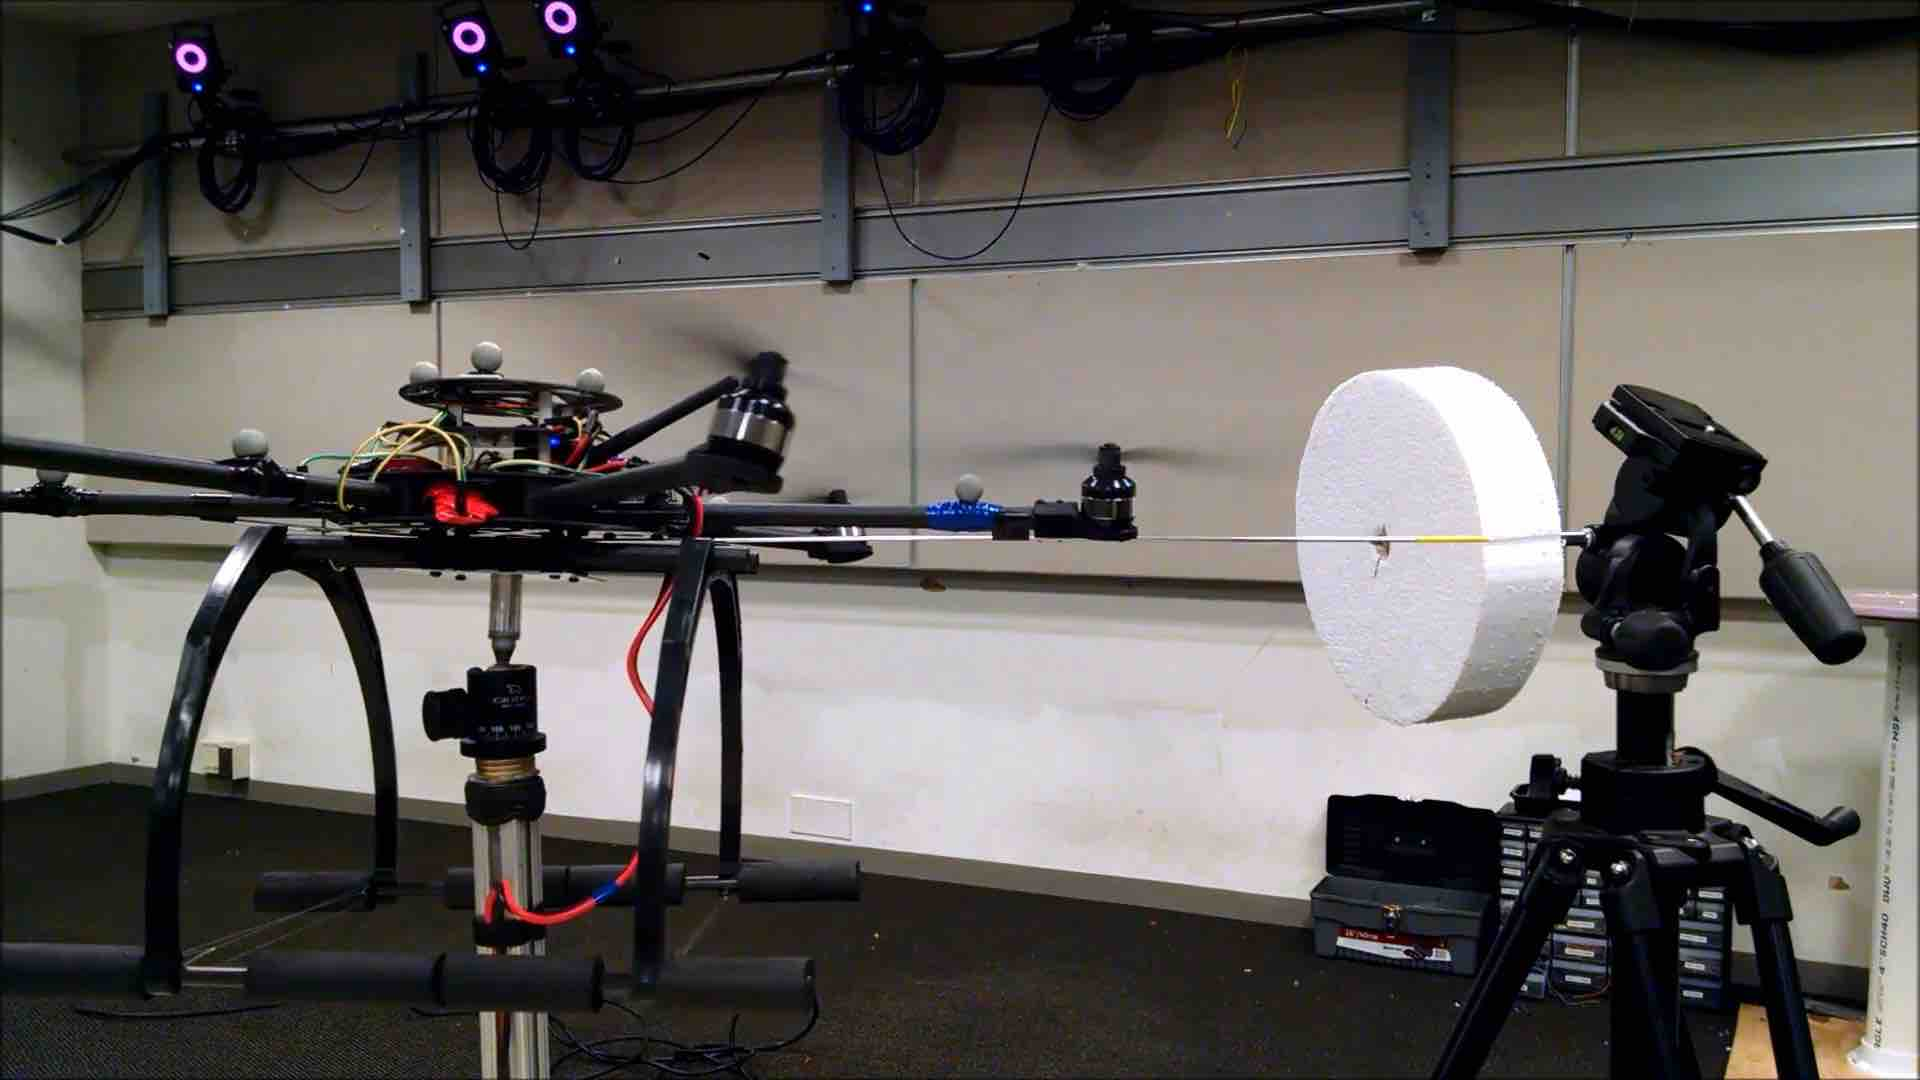
\includegraphics[height=0.7\textheight]{figures/2016ACC/hexrotor}}
\end{center}
\end{frame}   %-----------------------------%
